\documentclass[10pt]{report}

\usepackage{verbatim}
\usepackage{subcaption} % for subfigures
%\usepackage{amsthm} % for QED
%\usepackage{algpseudocode} % for pseudo-code
\usepackage{mathtools} % for \xRightarrow

\usepackage{listings} % for code
\lstset
{
	language=Matlab,
	frame=single,
	basicstyle=\footnotesize,
	numbers=left,
	stepnumber=1,
	showstringspaces=false,
	tabsize=4,
	breaklines=true,
	breakatwhitespace=false,
}

\usepackage{siunitx} % for scientific notation
% for `e' in scientific notation
\sisetup{output-exponent-marker=\ensuremath{\mathrm{e}}}

\usepackage{float} % for figure [H]
\usepackage{booktabs} % for tabular
\usepackage{caption} % for \caption*
\usepackage[export]{adjustbox} % for valign=t
\usepackage{array} % for column type m
\usepackage{verbatim}
\usepackage{graphicx}
\graphicspath{ {imgs/} }
\usepackage{fancyhdr}
\usepackage{amssymb}
\usepackage{amsmath}

%%%%%% Pagination
\setlength{\topmargin}{-.3 in}
\setlength{\oddsidemargin}{0in}
\setlength{\evensidemargin}{0in}
\setlength{\textheight}{9.in}
\setlength{\textwidth}{6.5in}

%Title page
\newcommand{\hwTitle}{Homework \#5}
\newcommand{\hwCourse}{Introduction to Computational Mathematics}
\newcommand{\hmwkClassInstructor}{Professor Shuwang Li}

\title{
	\vspace{2in}
	\textmd{\textbf{\hwCourse\\\hwTitle}}\\
	\vspace{0.3in}\large{\textit{\hmwkClassInstructor}}
	\vspace{3in}
}

%\title{Homework 1}
\author{\textbf{Zhihao Ai}}
\date{}

%Header setting.
\pagestyle{fancy}
\fancyhead[L]{Zhihao Ai}
\fancyhead[C]{Math 350}
\fancyhead[R]{Homework 5}
%%%%%%

%Custom commands.
\newcommand{\ds}{\displaystyle}
\newcommand{\eva}[2] {\left. #1 \right|_{#2}}
\newcommand{\dintt}[4] {\int_{#1}^{#2} #3 d#4}

\newcolumntype{C}{ >{\centering\arraybackslash} m{3em} }
\newcolumntype{D}{ >{\centering\arraybackslash} m{4em} }
\newcolumntype{N}{ >$ c <$}

\newcommand{\abs}[1] {\left| #1 \right|}
\newcommand{\norm}[2][\infty] {\left\Vert \mathbf{#2} \right\Vert_#1}

\begin{document}

\maketitle

\section*{Part 1. Reading Assignment}
%Read chapter 5.

\section*{Part 2. Fundamental Concepts/Ideas}
\begin{enumerate}
	\item 
	Given data
	\begin{table}[H]
		\centering
		\begin{tabular}{*{6}{N}} \toprule
			i & 1 & 2 & 3 & 4 & 5 \\ \midrule
			x_i & 1.0 & 1.4 & 1.8 & 2.2 & 2.6\\
			y_i & 0.931 & 0.473 & 0.297 & 0.224 & 0.618\\
			\bottomrule
		\end{tabular}
	\end{table}
	We can fit these data using a curve $y=p(x)=\frac{1}{a+bx}$ in the least square sense.
	\begin{enumerate}
		\item 
		Find coefficients $a$ and $b$. Hint: you can let $Y(x)=1/p(x)=a+bx$.
		
		Let $Y(x) = 1/p(x) = a + bx$, then $Y_i = 1/y_i$. To minimize $I(a, b) = \sum_i [(a+bx) - Y_i]^2$, let both $\partial{I}/\partial{a} = \partial{I}/\partial{b} = 0$ and we have
		\[
		\begin{cases}
		2\sum_i [(a + b x_i) - Y_i] \cdot 1 = 0\\
		2\sum_i [(a + b x_i) - Y_i] \cdot x_i = 0
		\end{cases}
		\Rightarrow
		\begin{cases}
		\sum_i a + (\sum_i x_i)b = \sum_i Y_i\\
		(\sum_i x_i)a + (\sum_i x_i^2)b = \sum_i x_i Y_i\\
		\end{cases}
		\]
		Below is the script that solves the equations:
		\lstinputlisting{hw5p1.m}
		The coefficients outputed is $a\approx 0.980376, b\approx 0.859535$.
		
		\item 
		Compute the residual $E = \sum_{i=1}^{5} [p(x_i) - y_i]^2$.
		
		The script above produces $E\approx 0.269785$.
		
		\item 
		Use Matlab to plot the curve $y=p(x)$ and $(x_i, y_i)$ on the same plot.
		
		\begin{figure}[H]
			\centering
			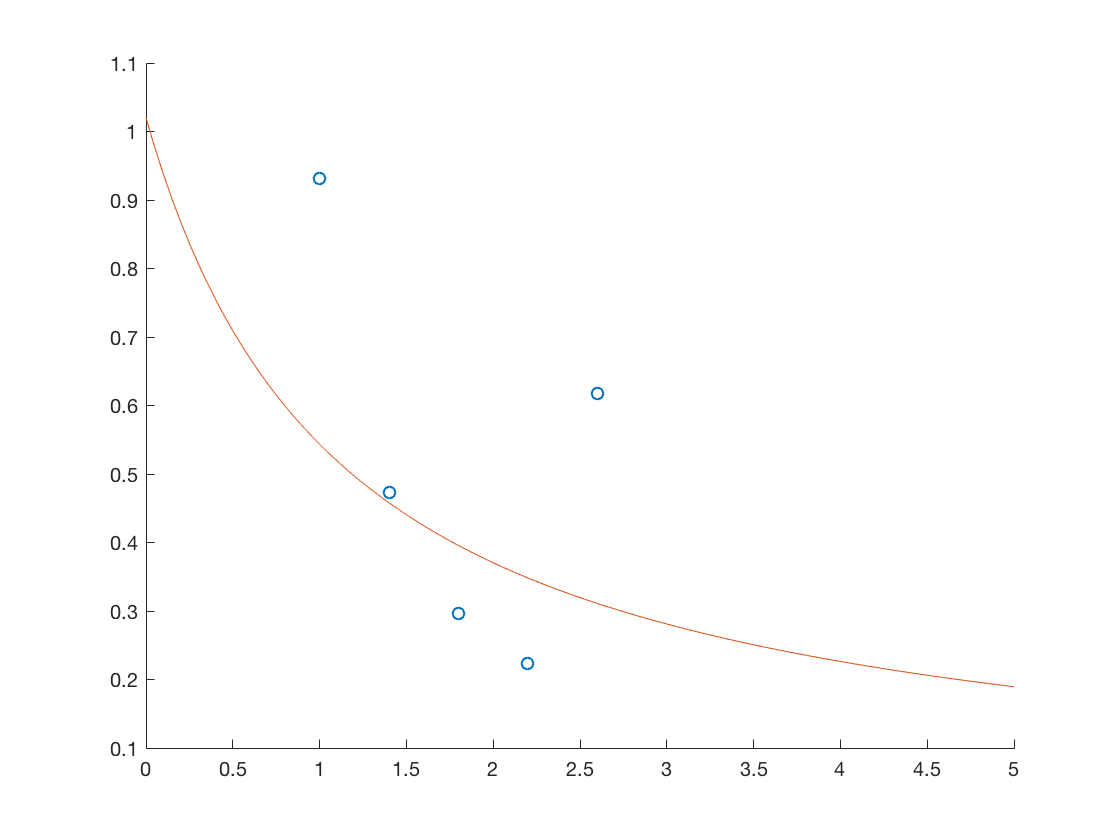
\includegraphics[width=0.5\linewidth]{hw5p1}
		\end{figure}
	\end{enumerate}
	\textit{Things learned:} Data fitting is about minimizing the error between the calculated curve and the data points. By setting the partial derivatives of each parameter to 0, we are able to minimize the error function. We can transform the curve function like $p(x) = \frac{1}{a+bx}$ into a form that is easy to take partial derivatives of. In the meantime, we also need to apply the same function to the original $y_i$'s to make the transformed question equivalent to the original one. In this question there is a outliner so the curve doesn't fit the first four well enough.

	\item 
	Given data
	\begin{table}[H]
		\centering
		\begin{tabular}{*{8}{N}} \toprule
			i & 1 & 2 & 3 & 4 & 5 & 6 & 7 \\ \midrule
			x_i & 0.2 & 0.3 & 0.4 & 0.5 & 0.6 & 0.7 & 0.8\\
			y_i & 3.16 & 2.38 & 1.75 & 1.34 & 1.00 & 0.74 & 0.56\\
			\bottomrule
		\end{tabular}
	\end{table}
	We can fit these data using a curve $y=q(x)=\beta e^{-\alpha x}$ in the least square sense.
	\begin{enumerate}
		\item 
		Find coefficients $\alpha$ and $\beta$. Hint: you can let $Y(x)=\ln y=\ln \beta - \alpha x$.
		
		Let $Y(x) = \ln{q(x)} = \ln{\beta} - \alpha x$, then $Y_i = \ln {y_i}$. To minimize $I(\alpha, \beta) = \sum_i [(\ln{\beta} - \alpha x_i) - Y_i]^2$, let both $\partial{I}/\partial{\alpha} = \partial{I}/\partial{\beta} = 0$ and we have
		\[
		\begin{cases}
		2\sum_i [(\ln{\beta} - \alpha x_i) - Y_i] \cdot x_i = 0\\
		2\sum_i [(\ln{\beta} - \alpha x_i) - Y_i] / \beta = 0
		\end{cases}
		\Rightarrow
		\begin{cases}
		(\sum_i x_i)\ln{\beta} - (\sum_i x_i^2)\alpha = \sum_i x_i Y_i\\
		\sum_i \ln{\beta} - (\sum_i x_i)\alpha = \sum_i Y_i
		\end{cases}
		\]
		Below is the script that solves the equations:
		\lstinputlisting{hw5p2.m}
		The coefficients outputed is $a\approx 2.888285, b\approx 5.631019$.
		
		\item 
		Compute the residual $E = \sum_{i=1}^{7} [q(x_i) - y_i]^2$.
		
		The script above produces $E\approx 0.000897$.
		
		\item 
		Use Matlab to plot the curve $y=q(x)$ and $(x_i, y_i)$ on the same plot.
		
		\begin{figure}[H]
			\centering
			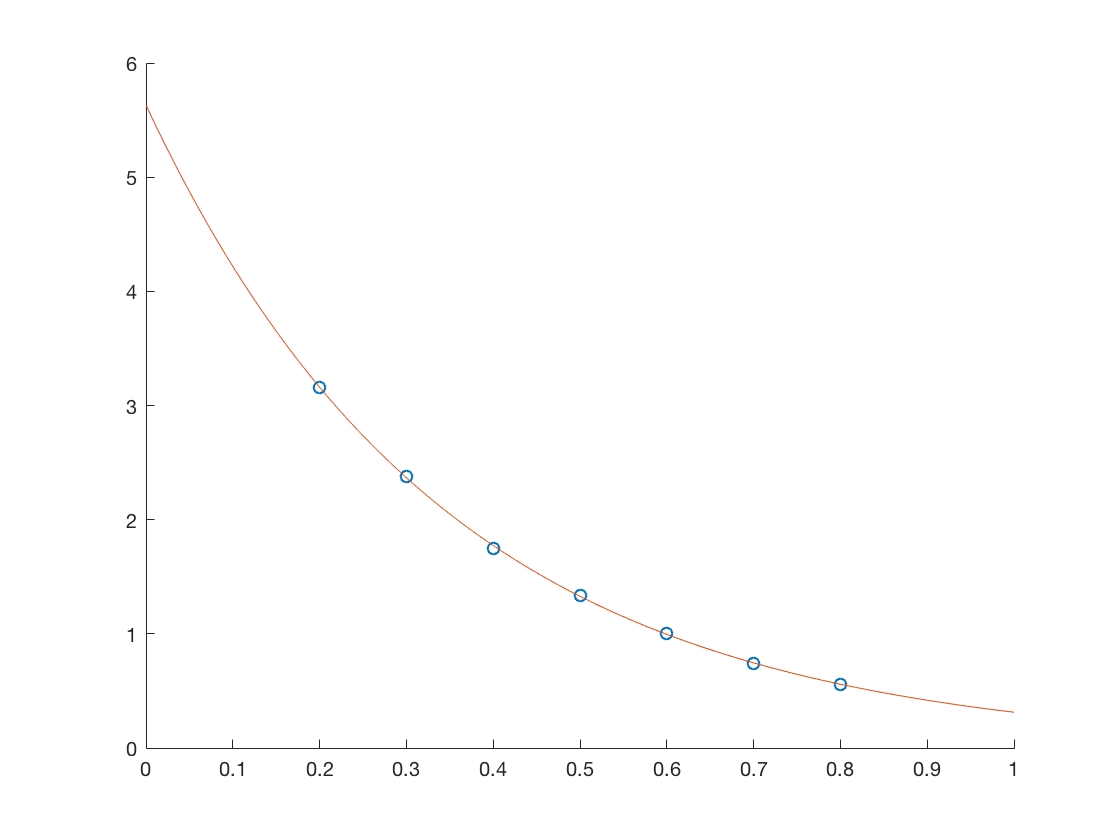
\includegraphics[width=0.5\linewidth]{hw5p2}
		\end{figure}
	\end{enumerate}
	\textit{Things learned:} The procedure is similar to problem 1. We need to set the partial derivatives to 0 and solve the equations to get the parameters. Since there is no outliner in this problem, the curve fits the data points well so the residual is quite small.
\end{enumerate}

\newpage

\section*{Part 3. Computer Assignments}
(Problem 5.8 @ Page 22) Given 25 observations, $y_k$, taken at equally spaced values of $t$.
\begin{enumerate}
	\item [(a)]
	Fit the data with a straight line, $y(t) = \beta_1 + \beta_2 t$, and plot the residuals, $y(t_k)-y_k$. You should observe that one of the data points has a much larger residual than the others. This is probably an \textit{outlier}.
	
	\lstinputlisting{hw5ca1a.m}
	\begin{figure}[H]
		\begin{subfigure}[b]{0.5\linewidth}
			\centering
			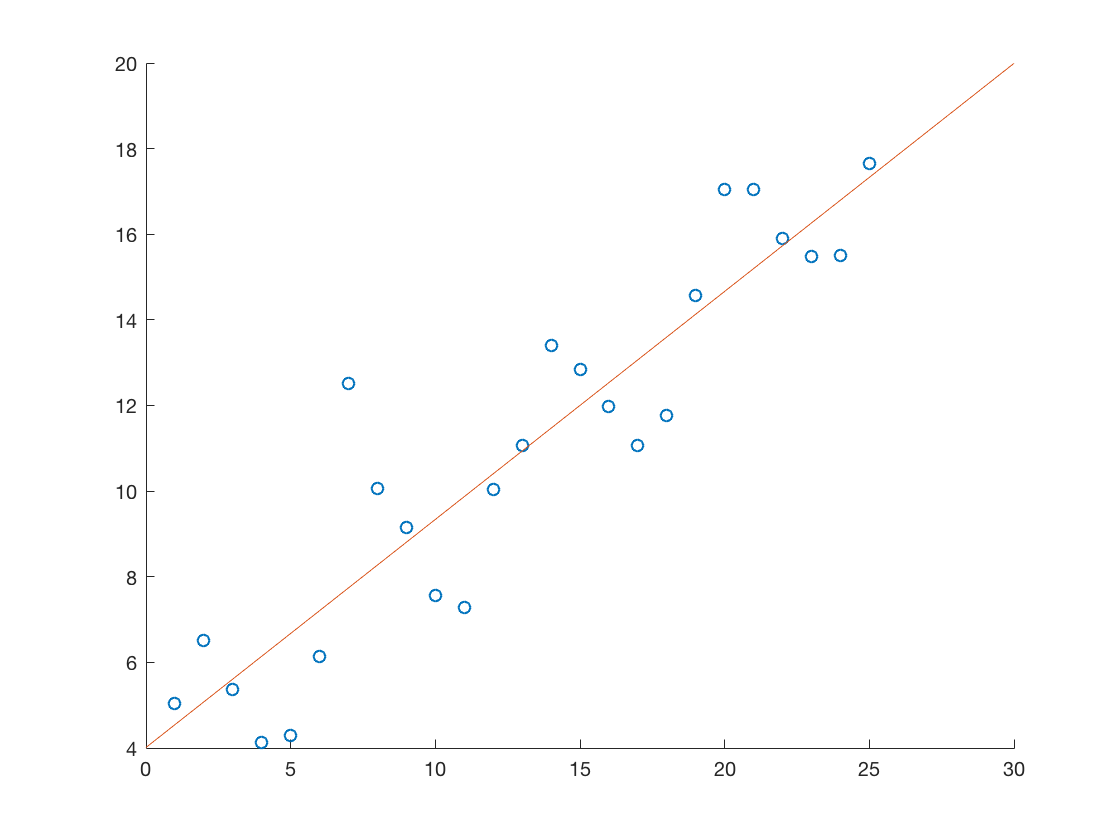
\includegraphics[width=\linewidth]{hw5ca1a_fit}
			\caption*{$y(t) = 4.012692 + 0.532643t$}
		\end{subfigure}
		\begin{subfigure}[b]{0.5\linewidth}
			\centering
			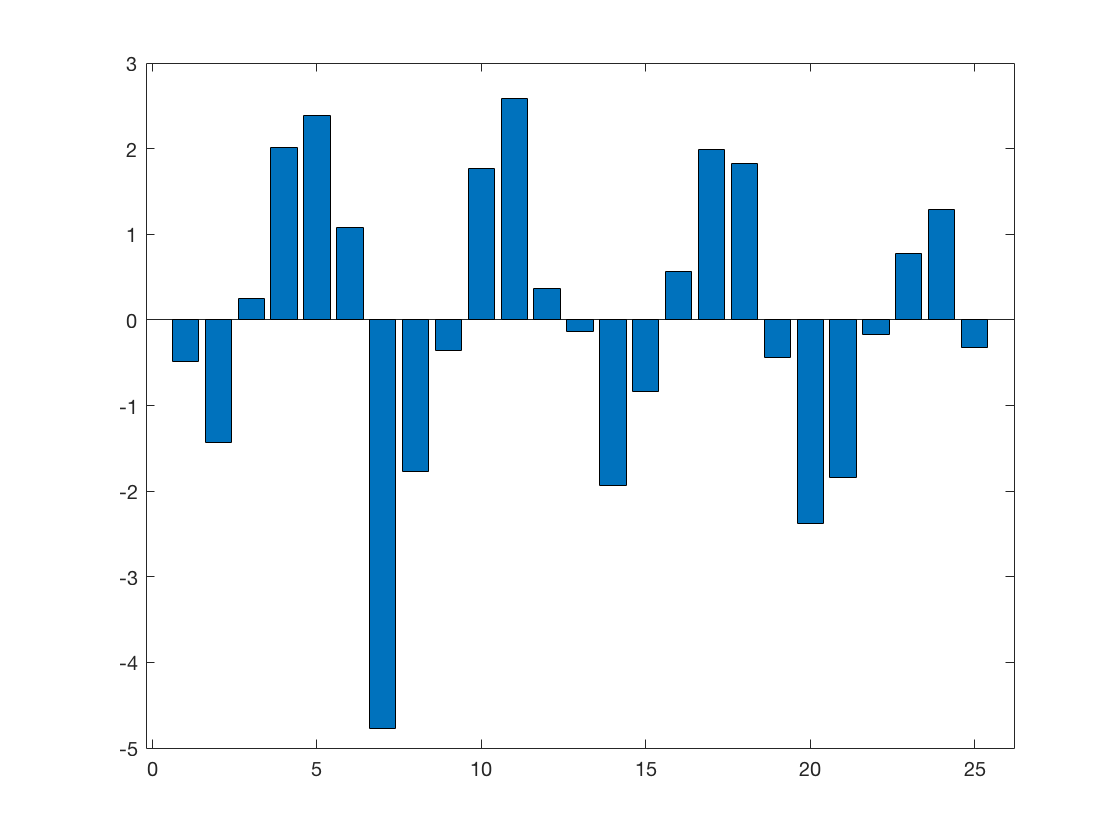
\includegraphics[width=\linewidth]{hw5ca1a_residual} 
			\caption*{$y(t_k)-y_k$}
		\end{subfigure}
	\end{figure}
	
	\item [(b)]
	Discard the outlier, and fit the data again by a straight line. Plot the residuals again. Do you see any pattern in the residuals?
	
	\begin{figure}[H]
		\begin{subfigure}[b]{0.5\linewidth}
			\centering
			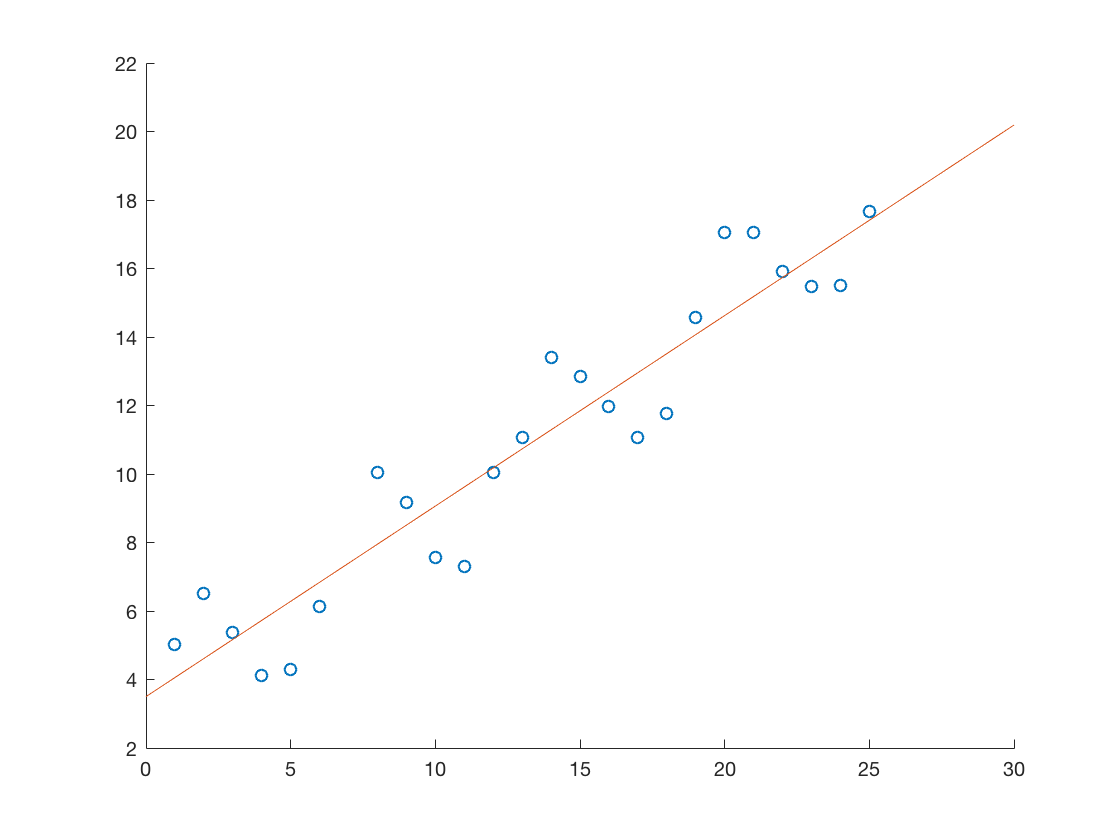
\includegraphics[width=\linewidth]{hw5ca1b_fit}
			\caption*{$y(t) = 3.500757 + 0.556271t$}
		\end{subfigure}
		\begin{subfigure}[b]{0.5\linewidth}
			\centering
			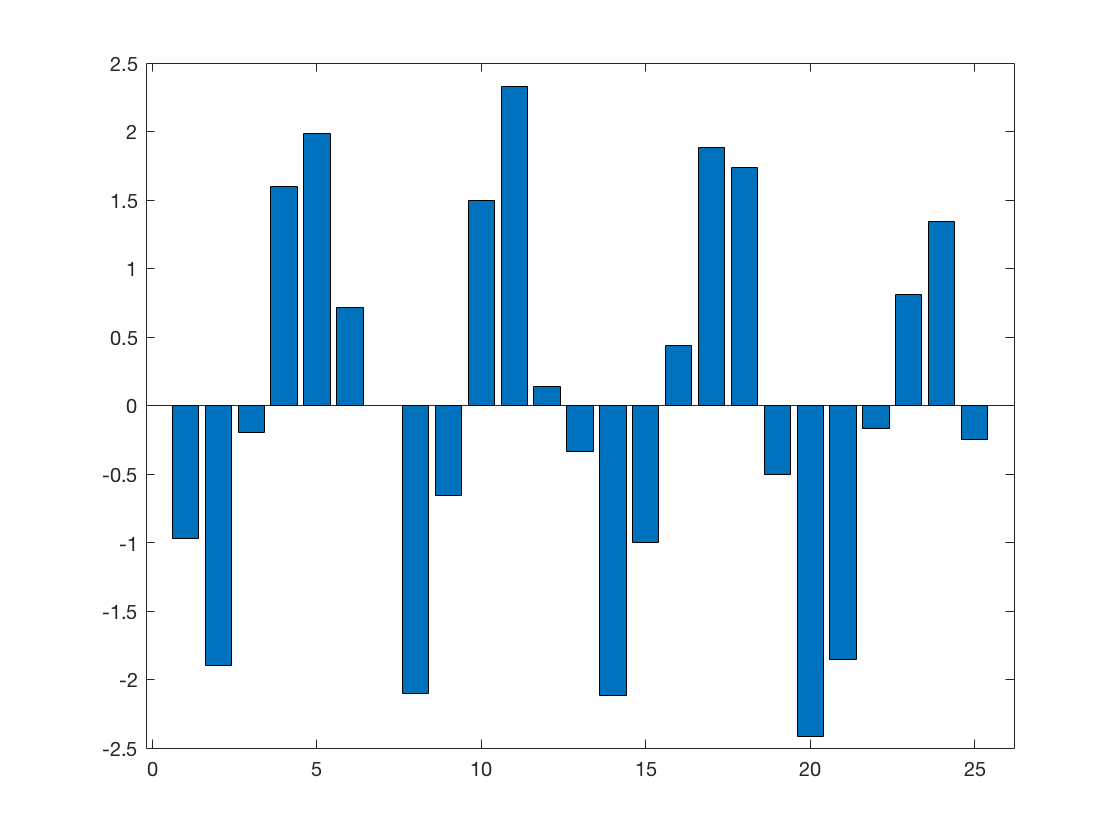
\includegraphics[width=\linewidth]{hw5ca1b_residual} 
			\caption*{$y(t_k)-y_k$}
		\end{subfigure}
	\end{figure}
	The residuals show a pattern of sin function.
	
	\item [(c)]
	Fit the data, with the outlier excluded, by a model of the form
	\[
	y(t) = \beta_1 + \beta_2 t + \beta_3 \sin t
	\]
	
	\lstinputlisting{hw5ca1c.m}
	According to the outputs, $y(t) = 3.289994 + 0.574871 t + 1.198019 \sin t$.
	
	\item [(d)]
	Evaluate the third fit on a finer grid over the interval $[0,26]$. Plot the fitted curve, using line style '-', together with the data, using line style 'o'. Include the outlier, using a different marker, '*'.
	
	\begin{figure}[H]
		\begin{subfigure}[b]{0.5\linewidth}
			\centering
			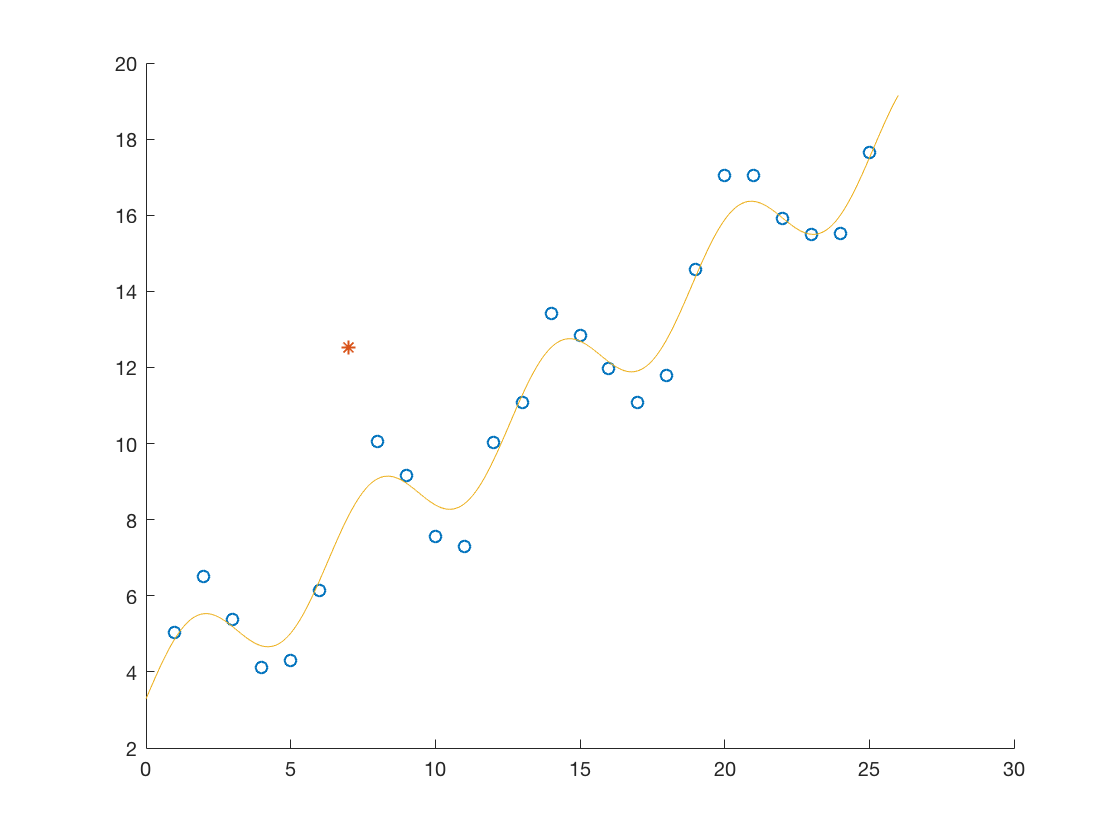
\includegraphics[width=\linewidth]{hw5ca1c_fit}
			\caption*{$y(t) = 3.289994 + 0.574871 t + 1.198019 \sin t$}
		\end{subfigure}
		\begin{subfigure}[b]{0.5\linewidth}
			\centering
			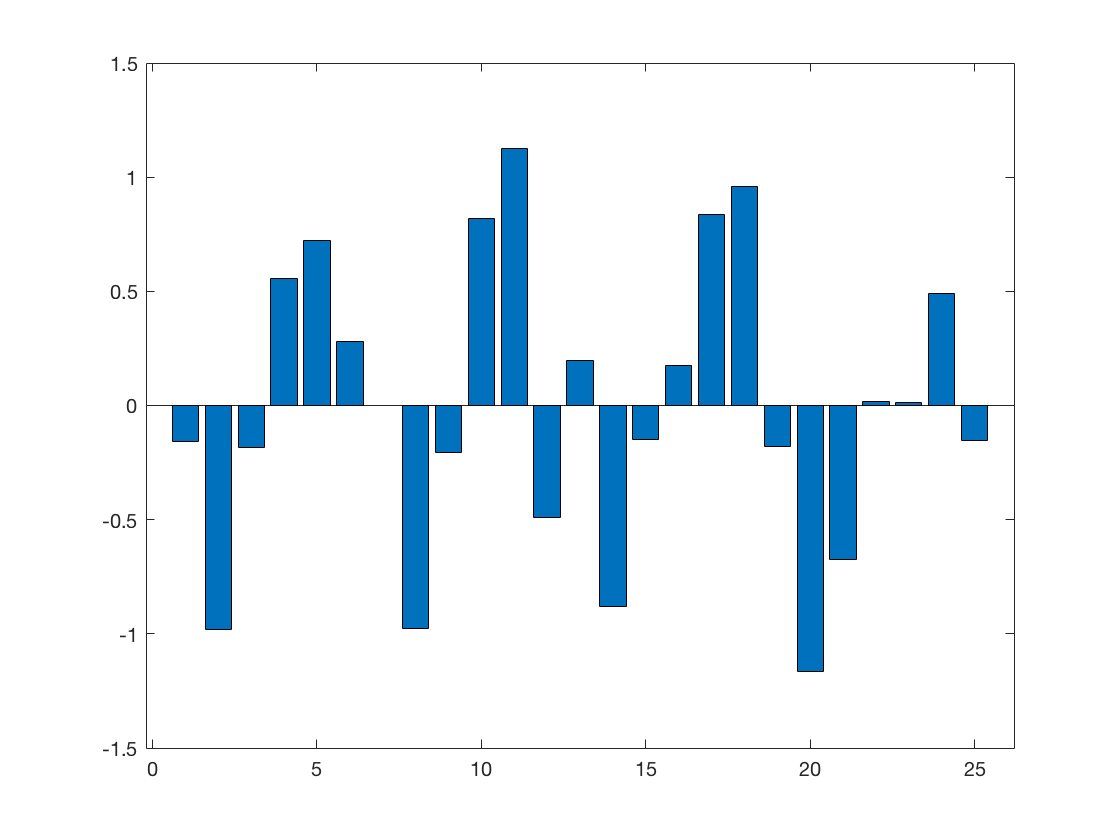
\includegraphics[width=\linewidth]{hw5ca1c_residual} 
			\caption*{$y(t_k)-y_k$}
		\end{subfigure}
	\end{figure}
	Excluding the outliner, the residual $E = \sum_{i=1}^{24} [y(t_i) - y_i]^2 \approx 9.682834$.
\end{enumerate}
\end{document}


